 
   %judul bisa diketik ulang
  \setstretch{1}%\small
  \begin{center}
      \textbf{\large \Title}\\
      \bigskip 
  \end{center}
  
  
  
  %Nama authors
   \begin{center}
     \bf \Author$^1$, Ade Romadhony$^2$
  \end{center}
  
  
  %Afiliasi dan email
   \begin{center}
      $^{1,2}$Fakultas Informatika, Universitas Telkom, Bandung\\
      $^1$nurcahyo@student.telkomuniversity.ac.id, $^2$aderomadhony@telkomuniversity.ac.id
  \end{center}
  
   
 %%% Abstrak Indonesia %%%%%%%%%%  
   
{\bf \parindent0pt \noindent\rule{\textwidth}{1pt}
Abstrak

Dokumen ini merupakan panduan penulisan jurnal Tugas Akhir (TA) di lingkungan Fakultas Informatika Universitas Telkom. Meskipun demikian, dimungkinan/dipersilahkan untuk pembimbing TA menggunakan struktur penulisan yang tidak sama persis dengan yang ada di dokumen ini. Panjang abstrak tidak lebih dari 200 kata dan diketik dalam ukuran huruf 10 pts. TA sebagai salah satu sarana latihan penulisan akademik dan memperjelas tulisan, abstrak dibagi menjadi empat paragraf atau sub-bagian. Setiap sub bagian bisa diberi judul yang digaris bawahi. Abstrak berisi apa, mengapa, bagaimana, dan hasil utama (kesimpulan).\\

\underline{\textit{Apa permasalahan pada topik}}. Yang juga menjelaskan latar belakang permasalahan topik. Sebaiknya tuliskan juga apa masukan dan keluaran secara sangat singkat. \\

\underline{\textit{Mengapa topik menarik atau penting}}. Sebisa mungkin tuliskan contohnya secara sangat singkat. Pada bagian ini sebaiknya ditulis juga \textit{apa masalah/kekurangan yang terjadi unt kondisi saat ini} (gap antara kondisi sekarang dengan yang diharapkan)? \\

\underline{\textit{Bagaimana solusinya}}. Jelaskan secara garis besar sistem solusi yang telah dilakukan. Biasanya penjelasan solusi ini merupakan yang terpanjang pada abstrak. \\

\underline{\textit{Hasil utama}}. Hasil utama dari eksperimen ditulis singkat dua-tiga kalimat. Akan lebih baik (optional), kalau dituliskan secara eksplisit kontribusi yang telah dihasilkan. Kontribusi bisa dituliskan diantara bagian solusi dan hasil eksperimen. \\

Pastikan abstrak pada jurnal TA tidak copas dari abstrak proposal TA. Pada abstrak proposal kadang ada kata \textit{akan}, seperti misalnya \textit{yang akan dilakukan}; sedangkan pada abstrak Jurnal TA tidak ada kata \textit{akan} spt itu. Tidak boleh ada sitasi pada abstrak. Pada abstrak tidak menggunakan penamaan, simbol atau istilah yang teknis, misalnya \textit{minsup} untuk menyatakan nilai support minimal.

 \bigskip
Kata kunci : merupakan kata-kata kunci yang menjelaskan isi tulisan, biasanya bisa diambil dari judul dan abstrak. Maksimal enam buah dan ditulis dengan huruf kecil, kecuali singkatan



%%% Abstrak English %%%%%%%%%%  



\noindent\rule{\textwidth}{1pt}
Abstract

The abstract should state briefly the general aspects of the subject and the main concolusions.  The length of abstract should bo no more than 200 word and  should be typed be with 10 pts.

 \bigskip
Keywords: keyword should be chosen that they best describe the contents of the paper and should be typed in lower-case, except abbreviation. Keyword should be no more than 6 word 

\noindent\rule{\textwidth}{1pt} }
   


%%%%%% isi paper %%%%

\section{Pendahuluan}

\noindent\textbf{Latar Belakang}

Riset pemrosesan bahasa alami untuk bahasa Indonesia saat ini masih terbilang sedikit.
Bahkan, masih banyak area riset yang belum tersentuh seperti contohnya
\textit{combinatory categorial grammar} (CCG).
Sementara itu, riset mengenai CCG untuk bahasa Inggris sudah cukup matang.
Adapun untuk bahasa lainnya (seperti bahasa Vietnam) sudah mulai menggunakan CCG di dalam
penelitiannya \citep{nguyen2019vietnamese}.
Agar dapat menerapkan CCG di dalam aplikasi yang dibangun, \textit{tools} seperti
CCG \textit{parser} dan CCG \textit{supertagger} harus tersedia terlebih dahulu.
Masing-masing dari \textit{tools} tersebut memerlukan \textit{dataset} agar dapat memberikan
hasil yang akurat.

Umumnya terdapat dua cara yang paling sering digunakan untuk mengembangkan CCG \textit{supertagger}
maupun CCG \textit{parser} bahasa lokal yaitu (1) membangun \textit{dataset} CCG \textit{supertag}
secara manual maupun semi-otomatis atau (2) melakukan transfer \textit{dataset} dari CCGbank
(atau dari sumber lainnya) ke dalam bahasa lokal dengan cara melakukan alih bahasa dan bila perlu
melakukan penyesuaian untuk \textit{supertag}-nya \citep{hockenmaier-steedman-2007-ccgbank}.
Proses pembangunan \textit{dataset} umumnya menggunakan bantuan \textit{annotation tool} agar
proses anotasinya menjadi lebih mudah.
Salah satu \textit{annotation tool} yang dapat digunakan adalah
CCGweb \citep{evang-etal-2019-ccgweb}.

Tugas akhir ini berusaha untuk membangun alat anotasi CCG baru dengan
UI/UX yang lebih baik dari CCGweb.
Selain itu, dengan bantuan NLTK alat anotasi ini dapat melakukan \textit{generate} untuk
CCG \textit{derivation}-nya kemudian pengguna juga dapat mengubah \textit{derivation}-nya
apabila diperlukan.
Tujuan dari dibangunnya alat anotasi CCG ini adalah untuk mempermudah proses anotasi yang
repetitif.
Selanjutnya, \textit{dataset} CCG pertama untuk bahasa Indonesia diharapkan dapat dipublikasikan.
\\


\noindent\textbf{Topik dan Batasannya}

Sub-bagian ini bisa juga dinamakan Perumusan Masalah atau Identifikasi Masalah. Untuk nama dalam Bahasa Inggris nama yang populer adalah \textit{Problem Statement} atau \textit{Problem Identification.}

Sub-bagian ini mempunyai fungsi sebagai penjelasan tentang topik TA yaitu apa isu/permasalahan yang akan dikerjakan. Untuk lebih memperjelas bisa juga disampaikan definisi atau pengertian. Penyampaian definisi dan penjelasan pada sub-bagian ini sebaiknya dilakukan dalam tulisan naratif dan informal (tanpa formula matematis) apa topik permasalahan yang telah dikerjakan untuk TA. Untuk mempermudah dalam menuliskan sub-bagian ini, dapat dipandang membuat penjelasan kata-kata kunci (pada abstrak) dan judul TA. Dengan penjelasan di sub-bagian ini, maka topiknya menjadi jelas bagi pembaca. Kalau digambarkan dalam sebuah algoritma, maka salah satu materi utama pada sub-bagian ini menjelaskan apa input dan output dari algoritma tersebut. Oleh karena itu, sangat dianjurkan untuk menerangkan apa input dan output, serta sebuah contoh kasusnya secara sangat singkat.

Sebutkan batasan pekerjaan yang ada. Batasan adalah kondisi-kondisi penyederhaan permasalahan, sehingga membuat pekerjaan semakin jauh dari ideal. Batasan masalah berisi pembatasan-pembatasan permasalahan agar menjadi lebih sederhana sehingga bisa/layak dikerjakan sebagai TA yang empat SKS dalam satu semester. Batasan diperlukan karena keterbatasan sumber daya saat pengerjaa TA, misalnya keterbatasan waktu pengerjaan yang hanya satu semester, keterbatasan data pendukung (misalnya tidak tersedianya korpus pengetahuan yang diperlukan) dan keterbatas kemampuan (misalnya untuk implementasi algoritma yang kompleks, dalam implementasinya diimplementasikan bentuk penyederhanaan). Salah satu ciri batasan yang bisa dipakai adalah bila bisa digunakan pada sub-bagian Saran (pada bagian Kesimpulan) agar TA berikutnya melonggarkan atau meniadakan batasan tersebut. Penyederhanaan yang dituliskan untuk batasan, antara lain meliputi data yang ditangani/digunakan, misalnya  jumlah data yang digunakan relatif sedikit, dan proses yang dikerjakan, misalnya ada satu subproses yang dikerjakan secara manual. Sebaiknya setiap batasan diberi alasan, misalnya jumlah data yang digunakan hanya 500 buah (relatif sedikit dibandingkan banyak penilitian unt topik sejenis) karena keterbatasan kemampuan komputer yang tersedia. Contoh lain, misalnya proses pelabelan peran semantik pada kalimat Bahasa Indonesia dilakukan secara manual, karena saat ini belum ditemukan alat bantu otomatis unt pelabelan peran semantik untuk Bahasa Indonesia yang efektif. Contoh batasan masalah yang tidak perlu misalnya sudah jelas tercerminkan pada judul.
\\


\noindent\textbf{Tujuan}

Sub-bagian Tujuan ini menerangkan kondisi apa yang hendak dicapai atau pertanyaan yang hendak dicari jawabannya. Sebisa mungkin tuliskan kondisi yang hendak dicapai yang terukur (bisa diukur dengan metrik evaluasi yang ditetapkan).  
Penulisan diupayakan dalam bentuk narasi (bukan berupa poin-poin).

Tujuan-tujuan yang ditetapkan menjadi bahan untuk menentukan skenario eksperimen yang dilakukan. atau dengan kata lain eksperimen dilakukan sesuai dengan tujuannya. Kemudian, kesimpulan pada jurnal TA harus selaras dengan tujuan. Hal ini bisa diilustrasikan pada Gambar 1 atau Tabel 1.
\begin{figure}[h!]
\centering
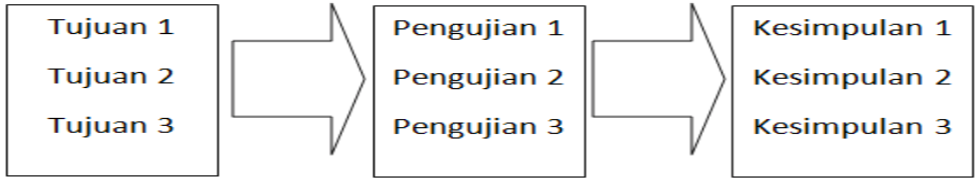
\includegraphics[scale=0.30]{Tujuan.png}
\caption{\textbf{Keterkaitan antara tujuan, pengujian dan kesimpulan}}
\label{fig:tujuan}
\end{figure}

\begin{table}[h!]
\caption{\textbf{Keterkaitan antara tujuan, pengujian dan kesimpulan}}
\label{table:1}%\bigskip
\centering
\begin{tabular}{| c | c  | c | c |} 
 \hline
 \textbf{No} & \textbf{Tujuan} & \textbf{Pengujian} & \textbf{Kesimpulan} \\ [0.5ex] 
 \hline
 1 & Tujuan 1 & Pengujian 1 & Kesimpulan 1 \\ 
 2 & Tujuan 2 & Pengujian 2 & Kesimpulan 2 \\ 
 3 & Tujuan 3 & Pengujian 3 & Kesimpulan 3 \\  [1ex] 
 \hline
\end{tabular}

\end{table}

\noindent \textbf{Organisasi Tulisan}

Pada sub-bagian ini dituliskan bagian-bagian selanjutnya (setelah Pendahuluan) pada jurnal TA ini, disertai penjelasan sangat singkat.



\section{Studi Terkait}

\noindent\textbf{Categorial Grammar}

Categorial Grammar (CG) merupakan sebuah istilah yang mencakup beberapa formalisme terkait yang diajukan
untuk sintaks dan semantik dari bahasa alami serta untuk bahasa logis dan matematis \citep{Steedman92catg}.
Karakteristik yang paling terlihat dari CG adalah bentuk ekstrim dari leksikalismenya di mana beban utama
(atau bahkan seluruh beban) sintaksisnya ditanggung oleh leksikon.
Konstituen tata bahasa dalam \textit{categorial grammar} dan khususnya semua leksikal diasosiasikan
dengan suatu \textit{type} atau \say{\textit{category}} (dalam \textit{category theory}) yang
mendefinisikan potensi mereka untuk dikombinasikan dengan konstituen lain untuk menghasilkan konstituen
majemuk.
\textit{Category} tersebut adalah salah satu dari sejumlah kecil \textit{category} dasar (seperti NP)
atau \textit{functor} (dalam \textit{category theory}).
Dalam hal ini, \textit{category} dapat diartikan sebagai \textit{syntactic type} dari suatu kata.

Secara formal, \textit{syntactic type} didefinisikan sebagai himpunan bagian dari suatu
\textit{semigroup} $M$ yang tunduk pada tiga operasi yaitu \ref{catg:syn:1},
\ref{catg:syn:2}, dan \ref{catg:syn:3} dimana $A$, $B$, dan $C$ merupakan himpunan bagian dari $M$
\cite{Lambek1988}. Adapun $A \cdot B$ dibaca $A$ \textit{times} $B$, $C/B$ dibaca $C$ \textit{over}
$B$, dan $A\backslash{}C$ dibaca $A$ \textit{under} $C$. Selanjutnya, dapat dilihat bahwasannya
untuk semua $A, B, C \subseteq M$ sehingga kita dapatkan \ref{catg:syn:4} dan \ref{catg:syn:5}.
Terakhir, persamaan \ref{catg:syn:6} dapat diabaikan apabila dihadapkan dengan
\textit{multiplicative system} yang tidak asosiatif. Sementara itu, apabila \textit{semigroup}-nya
merupakan sebuah \textit{monoid} dengan identitas $1$ maka kita dapatkan \ref{catg:syn:7} dimana
$I = \{1\}$.

\begin{align}
  \begin{split}\label{catg:syn:1}
    A \cdot B & = \{x \cdot y \in M \mid x \in A \land y \in B\}
  \end{split}\\
  \begin{split}\label{catg:syn:2}
    C/B & = \{x \in M \mid \forall_{y \in B} x \cdot y \in C\}
  \end{split}\\
  \begin{split}\label{catg:syn:3}
    A\backslash{}C & = \{y \in M \mid \forall_{x \in A} x \cdot y \in C\}
  \end{split}
\end{align}

\begin{align}
  \begin{split}\label{catg:syn:4}
    A \cdot B \subseteq C & \;\;\;\;\text{jika dan hanya jika}\;\;\;\; A \subseteq C/B
  \end{split}\\
  \begin{split}\label{catg:syn:5}
    A \cdot B \subseteq C & \;\;\;\;\text{jika dan hanya jika}\;\;\;\; B \subseteq A\backslash{}C
  \end{split}
\end{align}

\begin{align}
  \begin{split}\label{catg:syn:6}
    (A \cdot B) \cdot C = A \cdot (B \cdot C)
  \end{split}\\
  \begin{split}\label{catg:syn:7}
    I \cdot A = A = A \cdot I
  \end{split}
\end{align}

Ada beberapa notasi berbeda untuk \textit{category} dalam merepresentasikan \textit{directional}-nya.
Notasi yang paling umum digunakan adalah \say{\textit{slash notation}} yang dipelopori oleh Bar-Hilel,
Lambek, dan kemudian dimodifikasi dalam kelompok teori yang dibedakan sebagai tata bahasa
\say{\textit{combinatory}} \textit{categorial grammar} (CCG).
Sebagai contoh, \textit{category} $\text{(S$\backslash$NP)/NP}$ merupakan suatu \textit{functor} yang
memiliki dua buah notasi \textit{slash} yaitu $\backslash$ dan $/$.
Masing-masing notasi \textit{slash} tersebut merepresentasikan \textit{directionality} yang berbeda.
Notasi \textit{forward slash}, $/$, mengindikasikan bahwa argumen dari suatu \textit{functor}
$\text{X}/\text{Y}$ ada di bagian kanan atau dengan kata lain $\text{Y}$.
Adapun \textit{backward slash}, $\backslash$, mengindikasikan bahwa argumen dari suatu \textit{functor}
$\text{X}\backslash\text{Y}$ ada di bagian kiri atau dengan kata lain $\text{X}$.
Demikian itu, penggunaan notasi \textit{slash} yang tepat sangat penting dikarenakan hal ini dapat
mempengaruhi konstituen dari hasil \say{kombinasi} \textit{category}-nya.
\\


\noindent\textbf{Combinatory Categorial Grammar}\label{kajian-ccg}

Combinatory Categorial Grammar (CCG) merupakan salah satu formalisme tata bahasa yang gaya aturannya
diturunkan dari \textit{categorial grammar} dengan beberapa penambahan aturan dan istilah baru
\citep{Steedman96avery}.
Di CCG, \textit{category} dapat dipasangkan dengan \textit{semantic representation}.
Dalam hal ini, \textit{semantic representation} yang dimaksud adalah abstraksi fungsi lambda
(dalam \textit{lambda calculus}, \textit{lambda function}).
Sebagai contoh, \textit{category} $\text{(S$\backslash$NP)/NP}$ dapat dipasangkan dengan fungsi lambda
$\lambda{x. fx}$ sehingga dapat ditulis menjadi $\text{(S$\backslash$NP)/NP} : \lambda{x. fx}$.
Adapun pemetaan dari suatu token kata ke \textit{category}-nya menggunakan notasi $\vdash$.
Sebagai contoh, anggap saja kita memiliki kamus pemetaan seperti pada Gambar \ref{ccg:mapping:1}.
Apabila kita memiliki kalimat \say{Pamungkas dan Setyo menyukai rendang}, maka kita dapatkan:

\begin{figure}\centering\small
  \begin{align*}
    \text{Pamungkas} &\ \vdash\ \text{NP}:\ \so{pamungkas}\\
    \text{Setyo} &\ \vdash\ \text{NP}:\ \so{setyo}\\
    \text{dan} &\ \vdash\ \text{CONJ}:\ \lambda x.\lambda y.\lambda f.\ (f\ x) \land (f\ y)\\
    \text{menyukai} &\ \vdash\ \text{(S{$\backslash$}NP)/NP}:\ \lambda x.\lambda y.\ suka(y, x)\\
    \text{rendang} &\ \vdash\ \text{NP}:\ \so{rendang}
  \end{align*}
  \caption{Kamus yang memetakan token kata ke bentuk CCG \textit{lexicon}-nya.}
  \label{ccg:mapping:1}
\end{figure}

\begin{center}
  \bgroup
  \catcode`!=\active \def!{\upshape}
  \catcode`?=\active \def?#1{\makebox[0pt]{#1}}
  \catcode`^=\active \def^#1{\footnotesize{#1}}
  \catcode`*=\active \def*#1{\scriptsize{#1}}
  \tabbedShortstack{
    !^Pamungkas & & !^dan & & !^Setyo & & !^menyukai & & !^rendang &\\
    \TABcline{1,3,5,7,9}
    !^{$\text{NP}$} & &
      !^{$\text{CONJ}$} & &
      !^{$\text{NP}$} & &
      !^{$\text{(S$\backslash$NP)/NP}$} & &
      !^{$\text{NP}$} &\\
    !{*: \so{pamungkas}} & &
      !{*: $\lambda x.\lambda y.\lambda f.\ (f\ x) \land (f\ y)$} & &
      !{*: \so{setyo}} & &
      !{*: $\lambda x.\lambda y.\ suka(y, x)$} & &
      !{*: \so{rendang}} &
  }
  \egroup
\end{center}

Ada beberapa operasi yang dapat dilakukan dalam CCG. \textit{Operand} dari operasi
yang dimaksud adalah \textit{category}. Berdasarkan contoh di atas, akan ada tiga
operasi yang dijalankan yaitu \textit{coordination}, \textit{forward application},
dan \textit{type rising}.
Untuk mendapatkan hasil yang diinginkan, kita lakukan \textit{type rising} sebelum
\textit{forward application} di akhir.
Sehingga, kita dapatkan:

% \begin{center}
%   \bgroup
%   \catcode`!=\active \def!{\upshape}
%   \catcode`?=\active \def?#1{\makebox[0pt]{#1}}
%   \catcode`^=\active \def^#1{\footnotesize{#1}}
%   \catcode`*=\active \def*#1{\scriptsize{#1}}
%   \tabbedLongunderstack{
%     !^Pamungkas & & !^dan & & !^Setyo & & !^menyukai & & !^rendang &\\
%     \TABcline{1,3,5,7,9}
%     !^{$\text{NP}$} & &
%       !^{$\text{CONJ}$} & &
%       !^{$\text{NP}$} & &
%       !^{$\text{(S$\backslash$NP)/NP}$} & &
%       !^{$\text{NP}$} &\\
%     !{*: \so{pamungkas}} & &
%       !{*: $\lambda x.\lambda y.\lambda f.\ (f\ x) \land (f\ y)$} & &
%       !{*: \so{setyo}} & &
%       !{*: $\lambda x.\lambda y.\ suka(y, x)$} & &
%       !{*: \so{rendang}} &\\
%     \TABrule & \TABrule &
%       \TABrule & \TABrule &
%       \TABrule\CCGCOOR & &
%       \TABrule & \TABrule &
%       \TABrule\CCGFA &\\
%     & &
%       !?{^{$\text{NP}$}}
%       \ \ \ \ \ \ \ \ \ 
%       & & & &
%       \ \ \ \ \ \ \ 
%       !?{^{$\text{S$\backslash$NP}$}}
%       & & &\\
%     & &
%       ?{*: $\lambda f.\ (f\ \so{pamungkas}) \land (f\ \so{setyo})$}
%       \ \ \ \ \ \ \ \ \ 
%       & & & &
%       \ \ \ \ \ \ \ 
%       ?{*: $\lambda y.\ suka(y, \so{rendang})$}
%       & & &\\
%     \TABrule & \TABrule &
%       \TABrule & \TABrule &
%       \TABrule\CCGTR & &
%       & & &\\
%     & &
%       !?{^{$\text{S/(S$\backslash$NP)}$}}
%       \ \ \ \ \ \ \ \ \ 
%       & & & & & & &\\
%     & &
%       ?{*: $\lambda f.\ (f\ \so{pamungkas}) \land (f\ \so{setyo})$}
%       \ \ \ \ \ \ \ \ \ 
%       & & & & & & &\\
%     \TABrule & \TABrule &
%       \TABrule & \TABrule &
%       \TABrule & \TABrule &
%       \TABrule & \TABrule &
%       \TABrule\CCGFA &\\
%     & & &
%       !?{^{$\text{S}$}}
%       & & & & & &\\
%     & & &
%       ?{*: $suka(\so{pamungkas}, \so{rendang}) \land suka(\so{setyo}, \so{rendang})$}
%       & & & & & &
%   }
%   \egroup
% \end{center}

Berdasarkan hasil evaluasi tersebut, kita dapatkan \textit{query} \ref{ccg:query:1}
yang diperoleh dari kalimat \say{Pamungkas dan Setyo menyukai rendang}.
Demikian itu, komputer dapat melakukan komputasi berdasarkan \textit{query} yang telah diperoleh.
Kegiatan tersebut merupakan apa yang disebut dengan CCG \textit{parsing}.
Untuk dapat melakukan parsing, CCG \textit{lexicon} diperlukan.
Untuk mendapatkan CCG \textit{lexicon} kita dapat menggunakan CCG \textit{supertagger}
yang akan melakukan pelabelan suatu token kata ke CCG \textit{lexicon} berdasarkan
pemetaannya.

\begin{equation}\label{ccg:query:1}
  suka(\so{pamungkas}, \so{rendang}) \land suka(\so{setyo}, \so{rendang})
\end{equation}



\section{Sistem yang Dibangun}

Setelah bagian Pendahuluan dan bagian Studi Terkait, dijelaskan rancangan dan sistem atau produk yang dihasilkan. Penjelasan rancangan dan sistem/produk dituliskan dalam satu atau lebih bagian. Judul untuk bagian-bagian ini bisa menyesuaikan dengan topik TA. Bagian-bagian di sini tidak memuat teori secara umum, namun berisi rancangan dan sistem yang benar-benar telah dibuat atau dipakai. 

Sebaiknya judul tidak generik, seperti misalnya Sistem yang Dibangun; namun spesifik sesuai dengan topiknya. Contohnya untuk topik seputar deteksi plagiat, judul bagian-bagian ini misalnya bagian Praproses dan bagian Seeding, Extension dan Filtering. 

Uraikan data yang digunakan, sebaiknya disertai sampel data. Jelaskan juga metrik evaluasi yang dipakai serta alasan mengapa menggunakan/memilih metrik tersebut.

Bila diperlukan, informasi lebih detil tentang sistem atau produk yang dibangun bisa disampaikan pada lampiran. 

\section{Evaluasi}

Bagian ini berisi dua sub-bagian, yaitu Hasil Pengujian dan Analisis Hasil Pengujian. Pengujian dan analisis yang dilakukan selaras dengan tujuan TA sebagaimana dinyatakan dalam Pendahuluan.

\subsection{Hasil Pengujian}

Pertama, tampilkan hasil pengujian yang paling utama. Kemudian hasil-hasil yang lebih detil ditampilkan setelah hasil yang utama. Mengingat tinggi atau rendah, baik atau jeleknya hasil pengujian bersifat relatif, maka sangat dianjurkan ada pembanding (baseline) yang membandingkan dengan algoritma atau pendekatan yang dipilih untuk TA. Pembanding dijalankan pada lingkungan (termasuk data set) yang sama.

Pilih tabel atau jenis diagram yang sesuai untuk menampilkan hasil pengujian. 


\subsection{Analisis Hasil Pengujian}
 Analisis merupakan salah satu bagian yang penting untuk TA. Pada TA S1 tidak dituntut untuk mendapatkan hasil performasi yang lebih bagus dibandingkan dengan baseline yang populer, yang dituntut adalah membuat analisis yang lengkap. Menganalisis pengaruh kondisi-kondisi yang berbeda (seperti parameter, jenis data, threshold, dan sub-sistem) yang digunakan. 
 
 Cara sitasi adalah sebagai berikut: \citep{van2002fundamentals} untuk buku, \citep{ochoa2003hybrid} untuk \textit{paper}, dan \citep{Budi} untuk website.
   
   
\section{Kesimpulan}
 \noindent Bagian Kesimpulan memuat kesimpulan dan Saran (\textit{Future Work}), bisa dituliskan dalam poin-poin ataupun paragraf-paragraf. Semua poin kesimpulan diambil dari hasil pengujian dan analisis hasil pengujian sehingga tidak ada kesimpulan dari teori ataupun nalar semata. Sebagaimana sudah disebutkan pada bagian sebelumnya, pengujian dan analisis harus sesuai dengan tujuan TA. Jadi kesimpulan-kesimpulan yang dituliskan selaras dengan seluruh tujuan TA. 
 


\bibliographystyle{abbrv}
\bibliography{references}

\section*{Lampiran}

\noindent Lampiran dapat berupa detil data dan contoh lebih lengkapnya, data-data pendukung, detail hasil pengujian, analisis hasil pengujian, detail hasil survey, surat pernyataan dari tempat studi kasus, screenshot tampilan sistem, hasil kuesioner dan lain-lain.